\begin{figure}[h!]
    \centering
    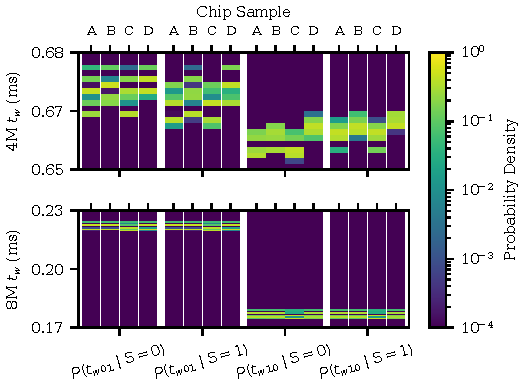
\includegraphics[width=0.95\linewidth]{fig/images/pdf/single-bit-buffer-scans-heat-bars.pdf}
    \vspace{-.5cm}
    \caption{Write latency distributions for 1-bit transitions within uniformly initialized 256-byte segments measured on 4 4M samples (top) and 4 8M samples (bottom). Each heatmap bar is a collapsed histogram colored according to the log-probability of observing a $t_w$ in each $\Delta t$-sized bin. $t_{w01}$ and $t_{w10}$ latencies correspond to data word transitions with a DHD of $\left(1,0 \right)$ and $\left(0,1\right)$, respectively. \label{fig:1b-buff-scan}}
\end{figure}